\begin{frame}{Training as Optimization}
    \begin{itemize}
        \item<1-> we learned that the goal of training is to minimize a loss function (and a regularization term)
        \begin{equation*}
            \hat{\Theta} =\text{argmin}_{\Theta} \left( \mathcal{L}(\hat{y},y)  + \lambda R(\Theta) \right)
        \end{equation*}
        \item<2-> training = Solving an optimization problem
        \item<3-> how to find parameter values that minimize loss?
    \end{itemize}
\end{frame}
\begin{frame}{Gradient-based Optimization}
   
  \only<1-1>{
    \begin{figure}
        \centering
        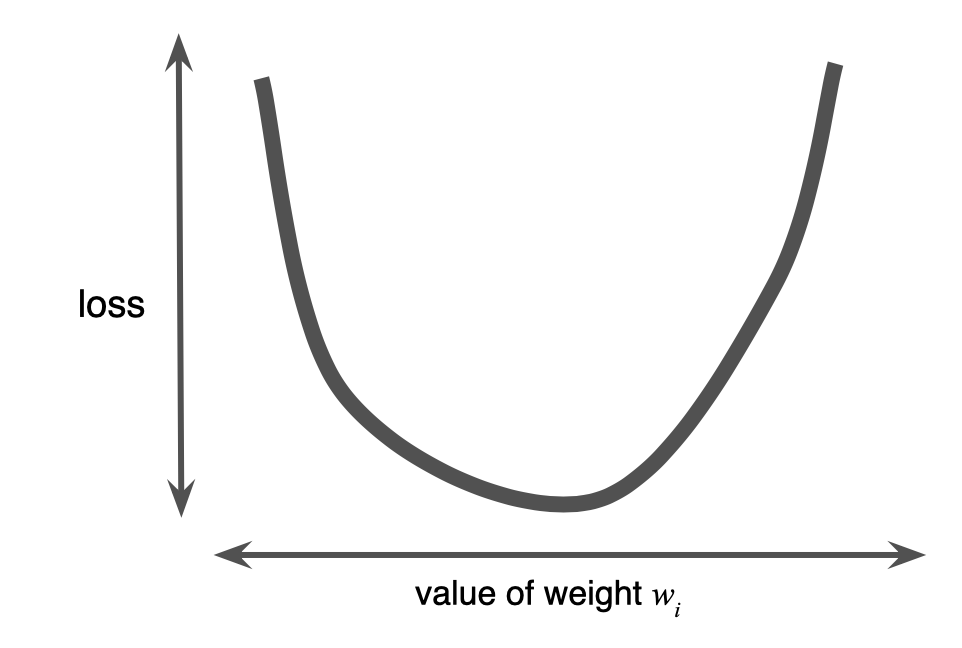
\includegraphics[scale=0.2]{final/figures/sgd1.png}
    \end{figure}
    }
    \only<2-2>{
        \begin{figure}
        \centering
        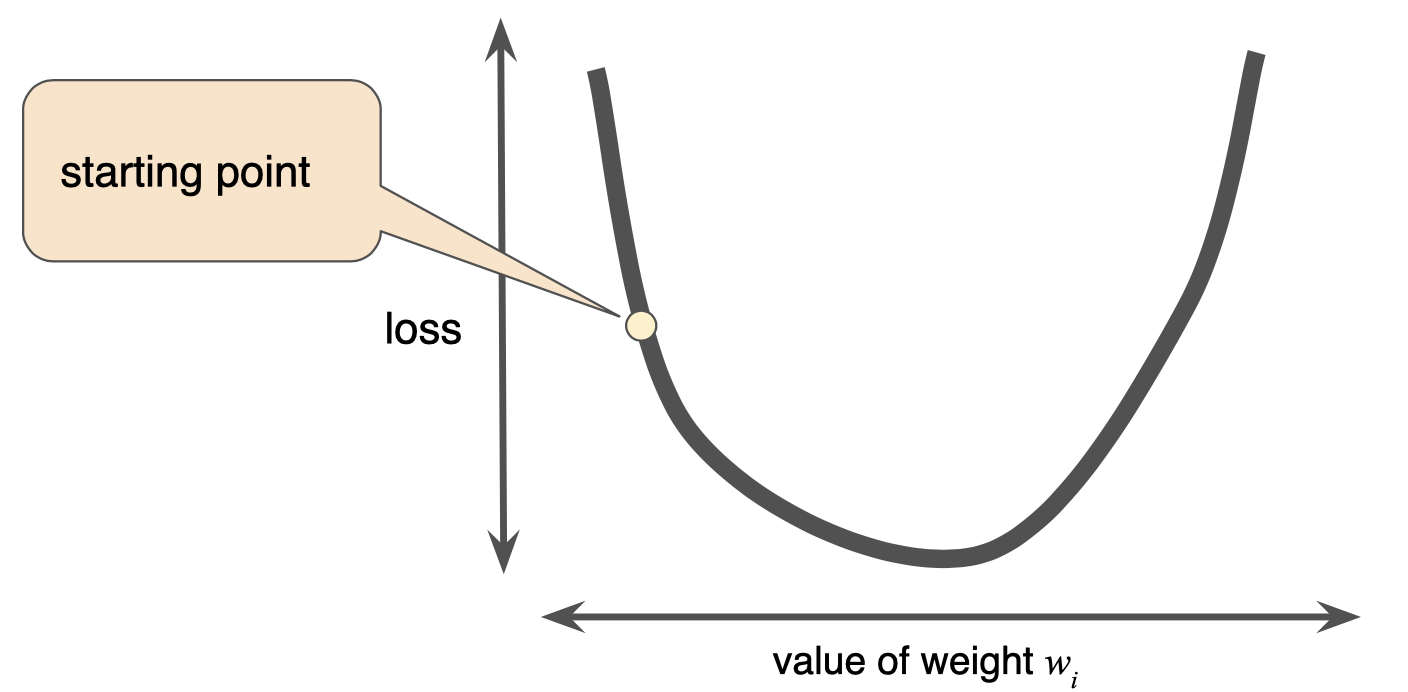
\includegraphics[scale=0.2]{final/figures/sgd2.png}
    \end{figure}
    }
    \only<3-3>
    {
      \begin{figure}
        \centering
        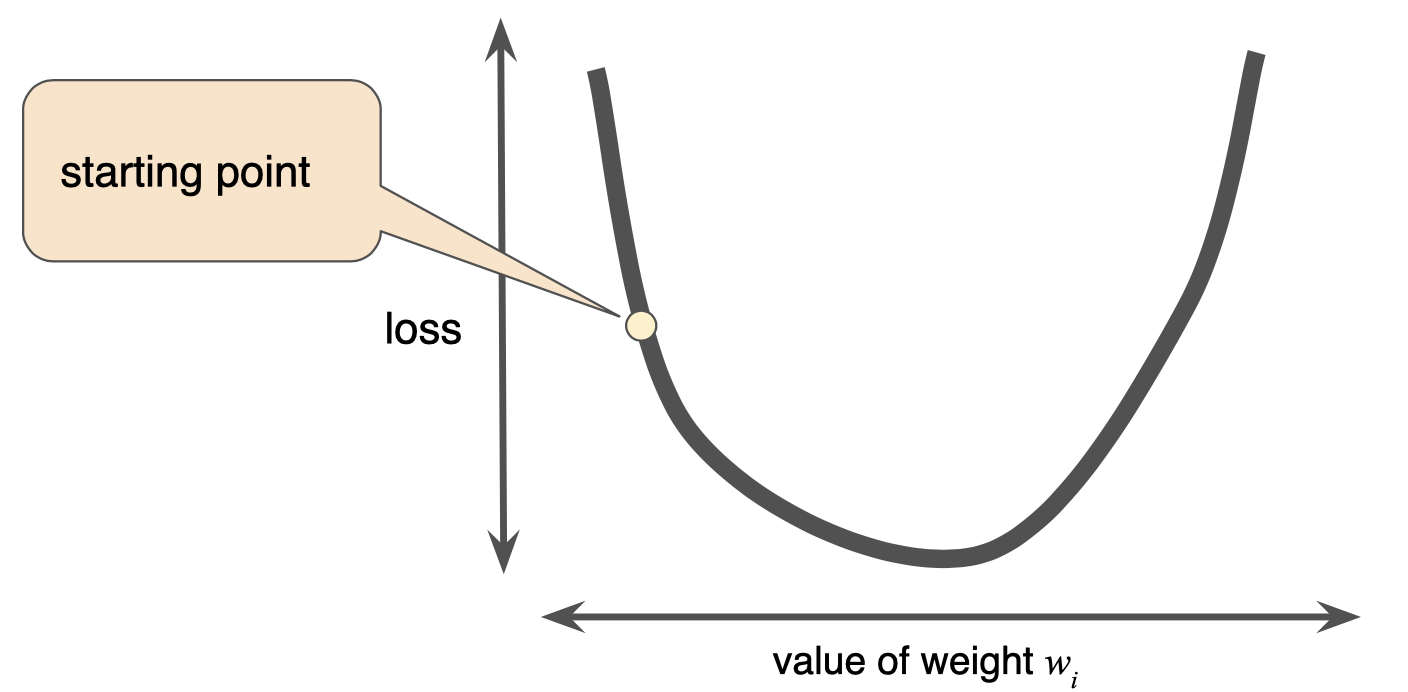
\includegraphics[scale=0.2]{final/figures/sgd2.png}
    \end{figure}      
    }
    \only<4-4>
    {
     \begin{figure}
        \centering
        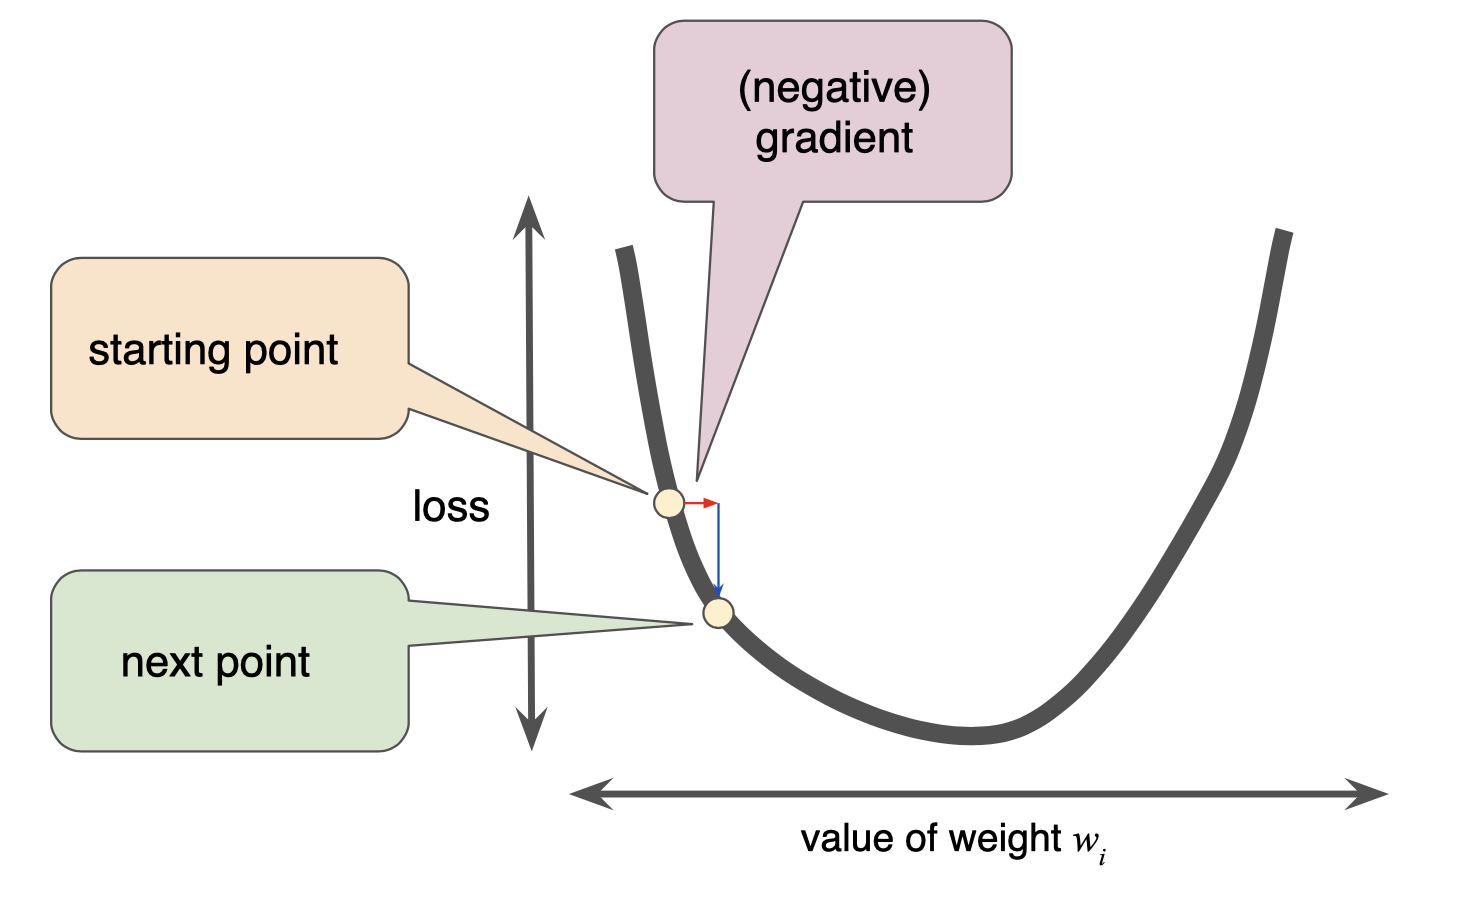
\includegraphics[scale=0.2]{final/figures/sgd4.png}
    \end{figure}
    }
\vspace*{\fill}
\textit{\tiny{(Taken from: 
\url{https://developers.google.com/machine-learning/crash-course/reducing-loss/gradient-descent})}}
   
\end{frame}
\begin{frame}{Gradient-based Optimization}
    \begin{itemize}
        \item<1-> we repeatedly compute an estimate of the loss over the training set
        \item<2-> we compute the gradients of the parameters‚ with respect to the loss estimate
        \item<3-> we move the parameter values in the opposite directions of the gradient
    \end{itemize}
\end{frame}
\begin{frame}{(Online) Stochastic Gradient Descent}
\centering
\begin{figure}
    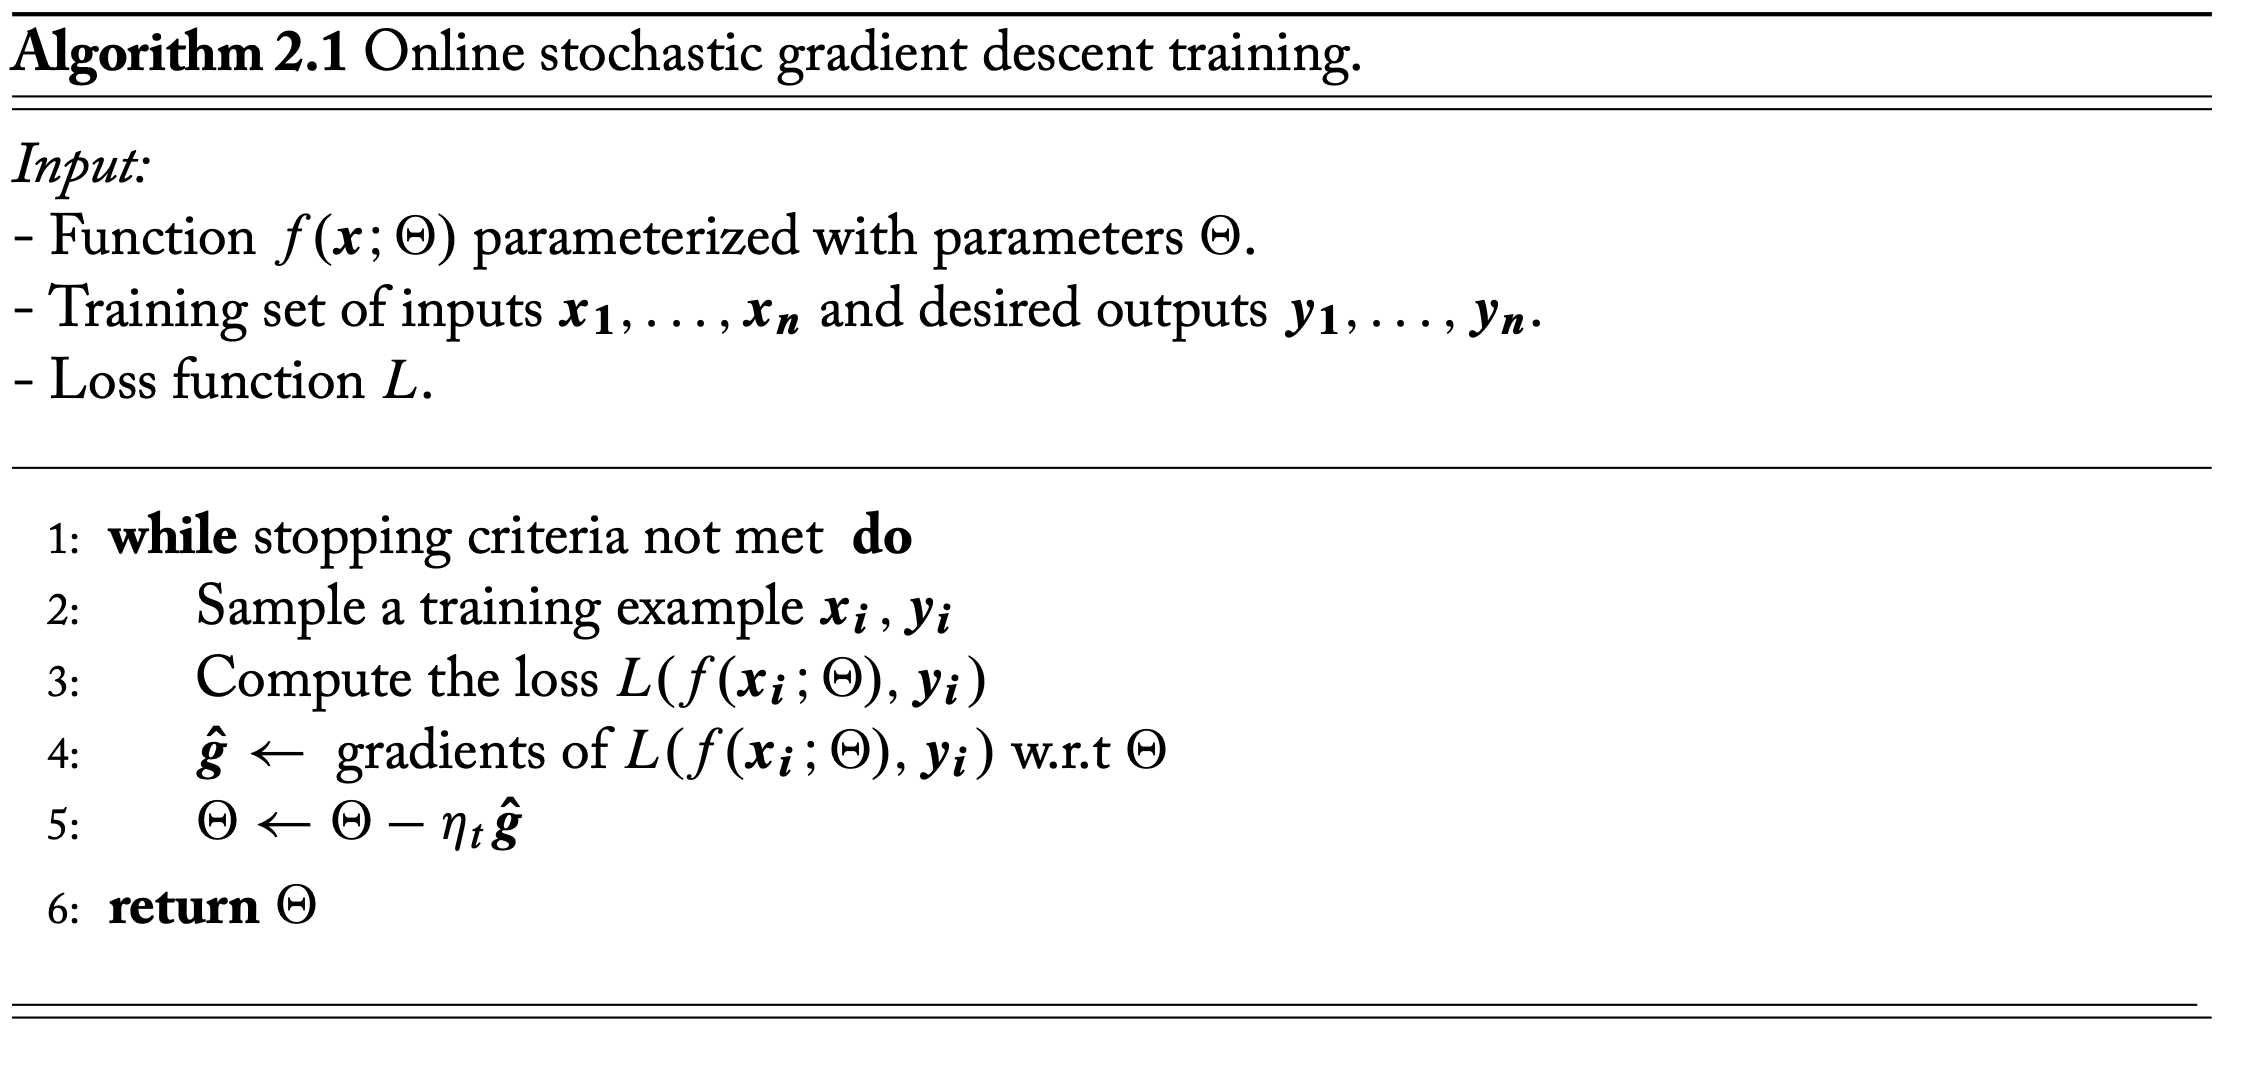
\includegraphics[scale=0.25]{final/figures/sgd.png}
\end{figure}
\vspace*{\fill}
\textit{\tiny{(Taken from: Neural Network Methods for Natural Language Processing, Yoav Goldberg)}}
\end{frame}
\begin{frame}{\Large{(Minibatch) Stochastic Gradient Descent}}
\centering
\begin{figure}
    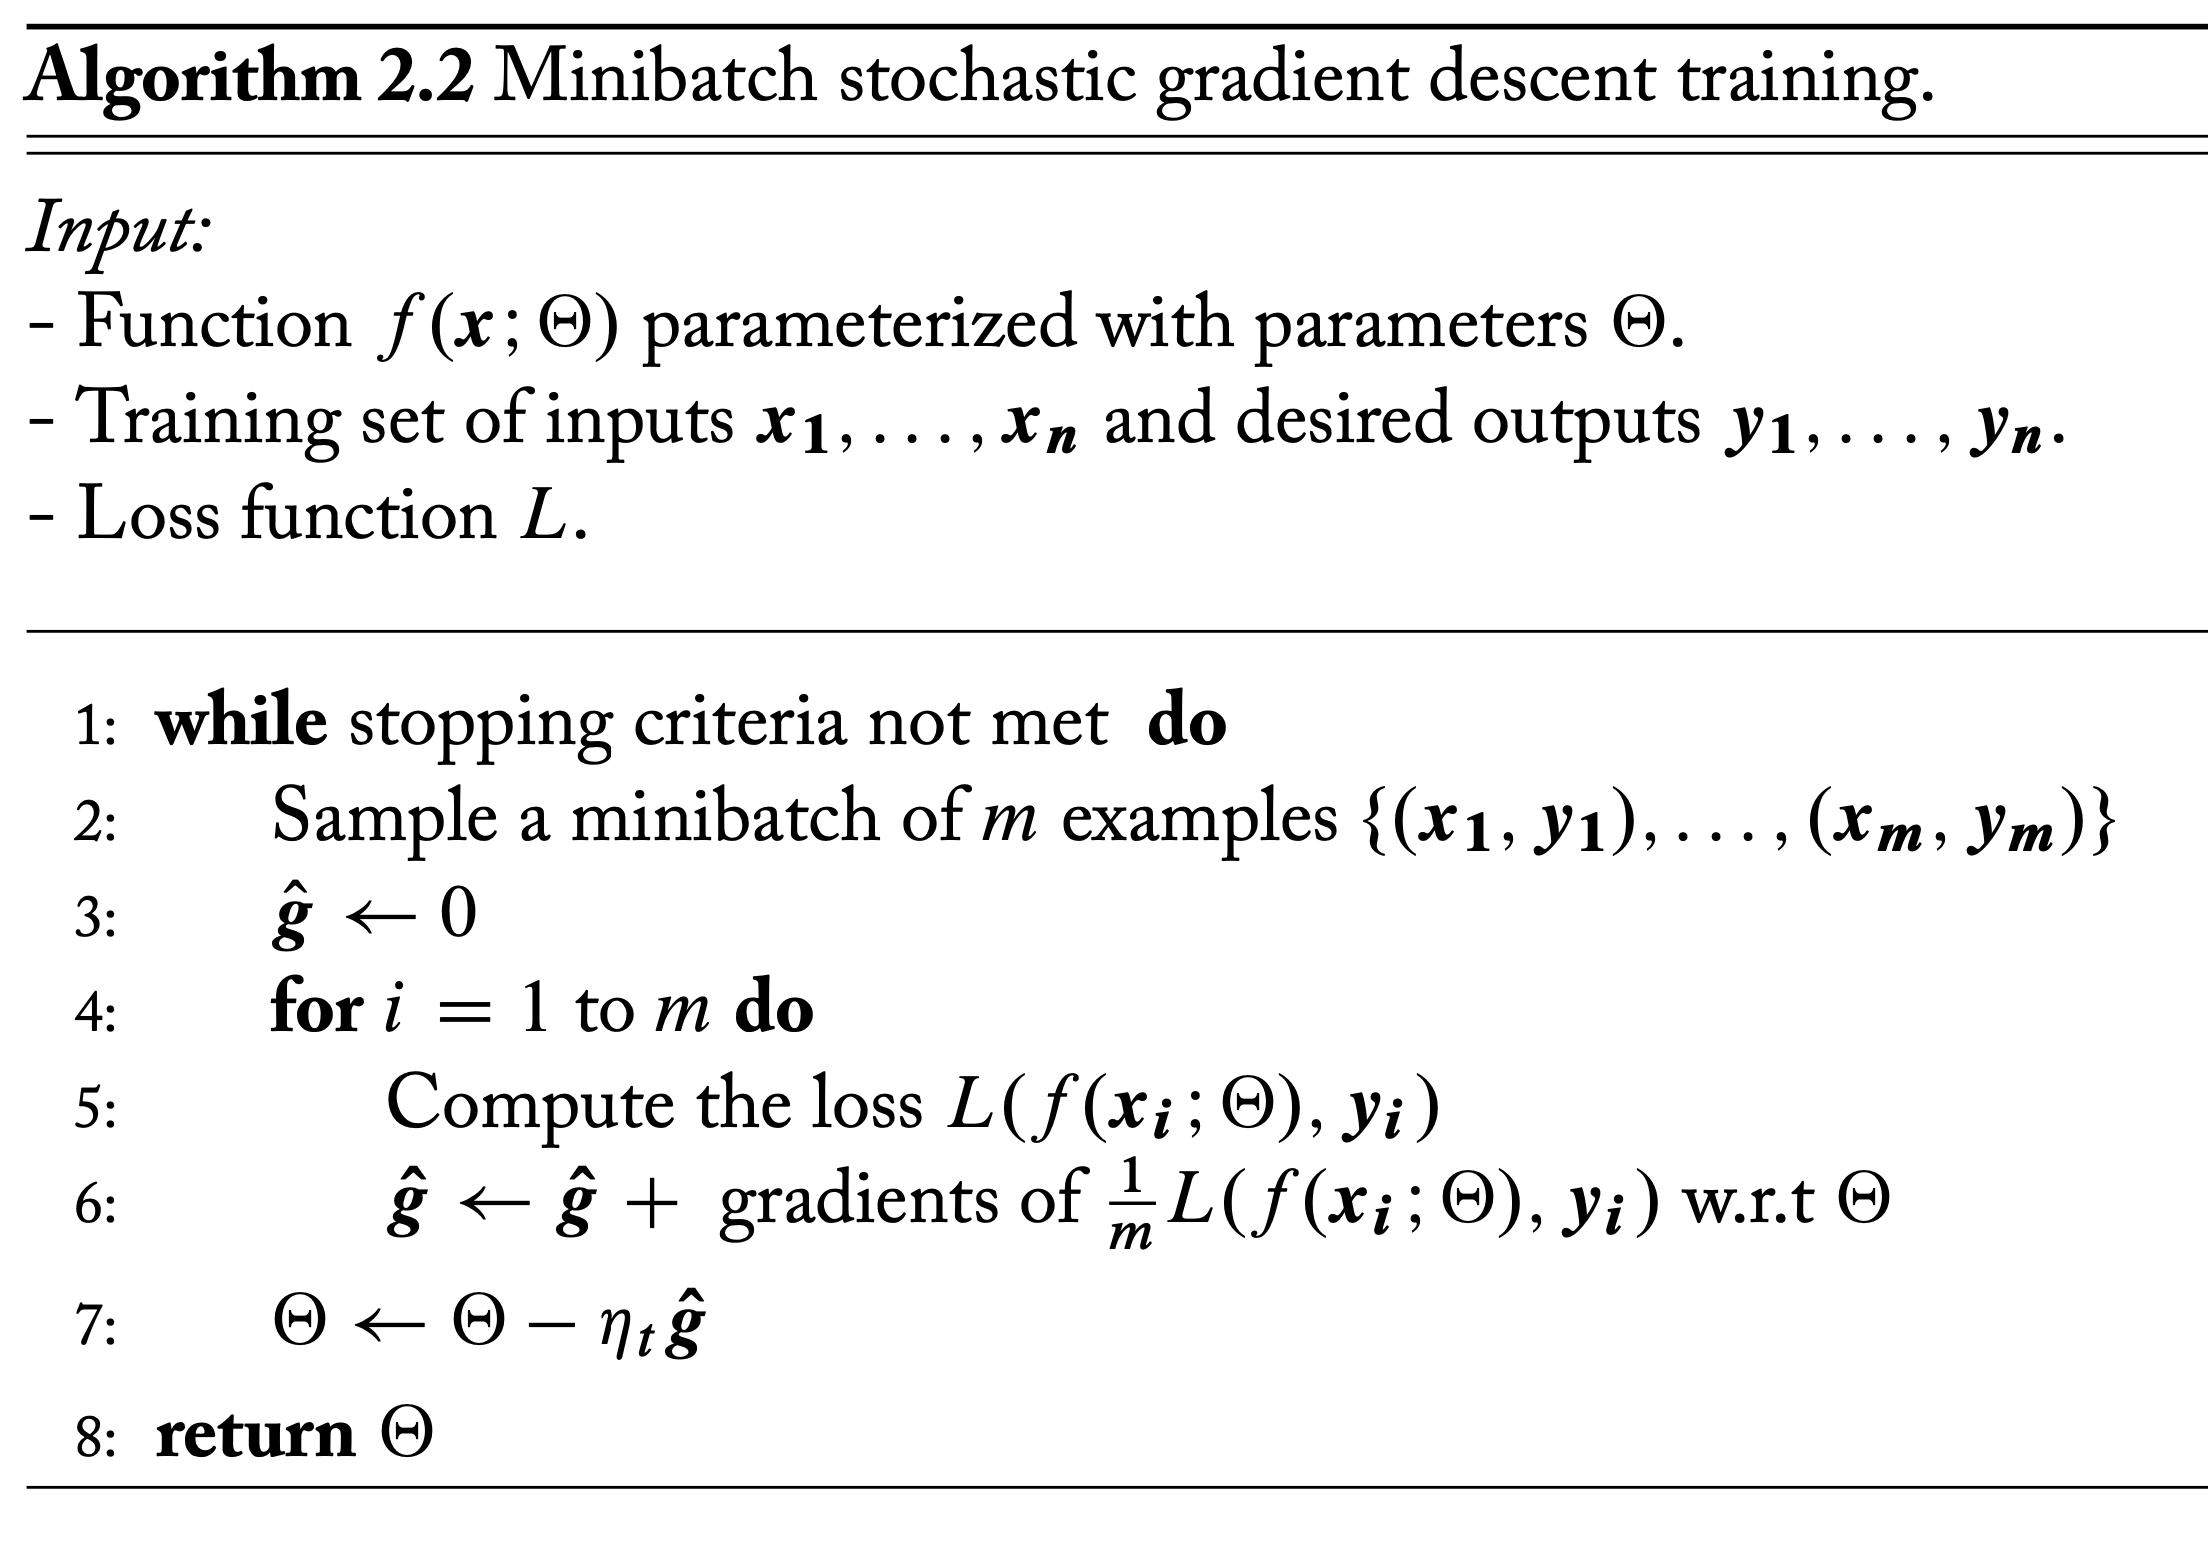
\includegraphics[scale=0.20]{final/figures/msgd.png}
\end{figure}
\vspace*{\fill}
\textit{\tiny{(Taken from: Neural Network Methods for Natural Language Processing, Yoav Goldberg)}}
\end{frame}
\begin{frame}{Why Minibatch SGD?}
    \begin{itemize}
        \item<1-> it's not expensive: while computing loss function gradient on all training set can be computationally
expensive 
        \item<2-> it converges faster to a good solution than full-batch learning, in which we use all training set to compute gradient
        \item<3-> smaller mini-batch sizes lead often to better solutions (generalize better)
    \end{itemize}
\end{frame}
\begin{frame}{Stochastic Gradient Descent (SGD)}
    \begin{itemize}
        \item<1-> gradient descent does not always lead to best solutions
        \begin{figure}
            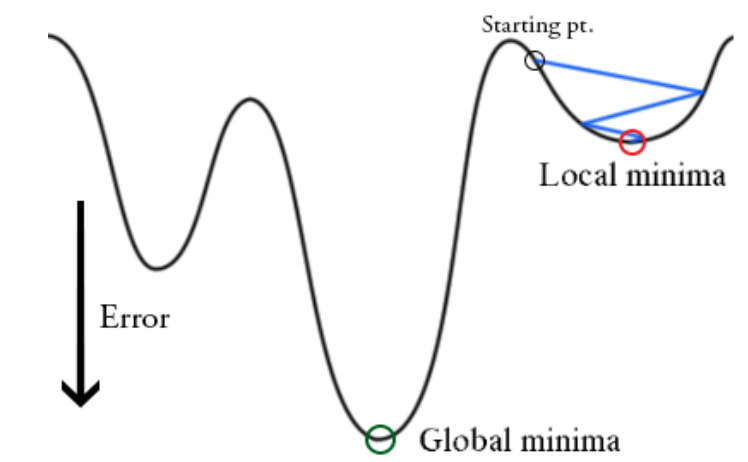
\includegraphics[scale=0.3]{final/figures/sgd5.png}
        \end{figure}
        \item<2-> why? 
        \item<3-> SGD is sensitive to the learning rate and initial parameter values (starting point)
    \end{itemize}
\end{frame}
\begin{frame}{Small Learning Rate}
         \begin{figure}
        \centering
         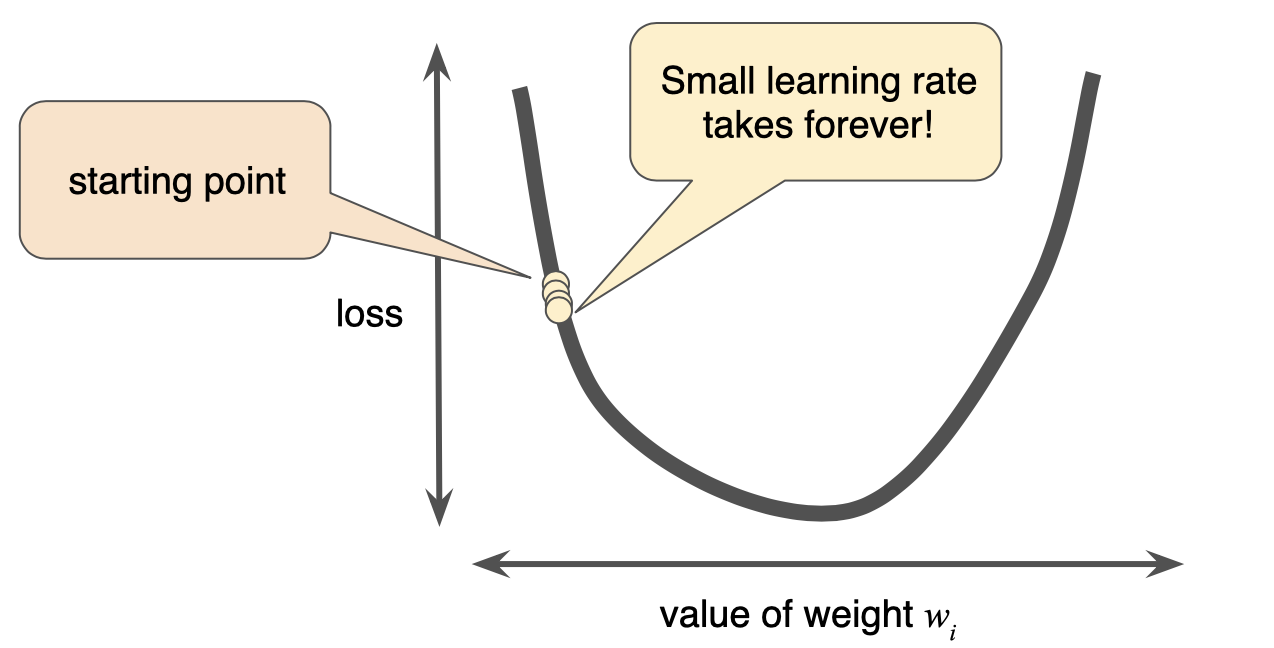
\includegraphics[scale=0.4]{final/figures/small_lr.png}
        \end{figure}
\vspace*{\fill}
\textit{\tiny{(Taken from: 
\url{https://developers.google.com/machine-learning/crash-course/reducing-loss/gradient-descent})}}     
\end{frame}
\begin{frame}{Large Learning Rate}
         \begin{figure}
        \centering
          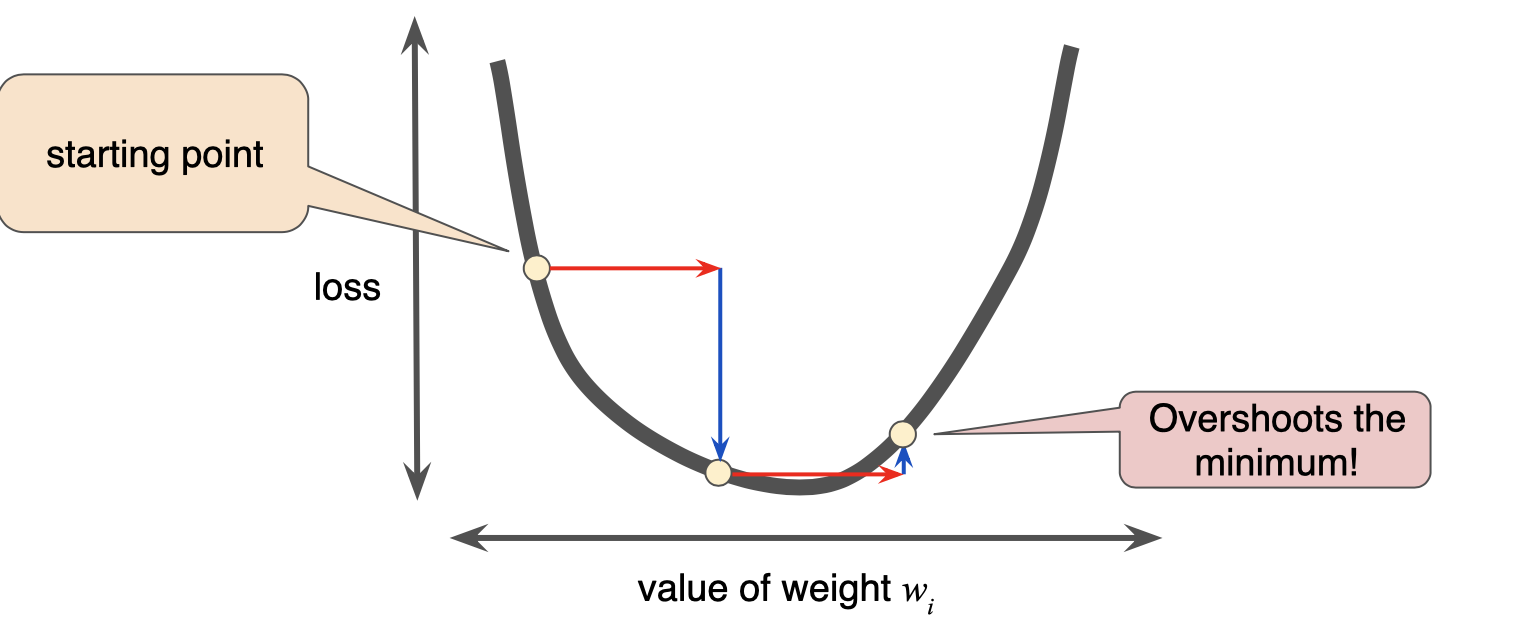
\includegraphics[scale=0.4]{final/figures/large_lr.png}
        \end{figure}
\vspace*{\fill}
\textit{\tiny{(Taken from: 
\url{https://developers.google.com/machine-learning/crash-course/reducing-loss/gradient-descent})}}
\end{frame}
\begin{frame}{Adaptive Learning Rate}
         \begin{figure}
        \centering
        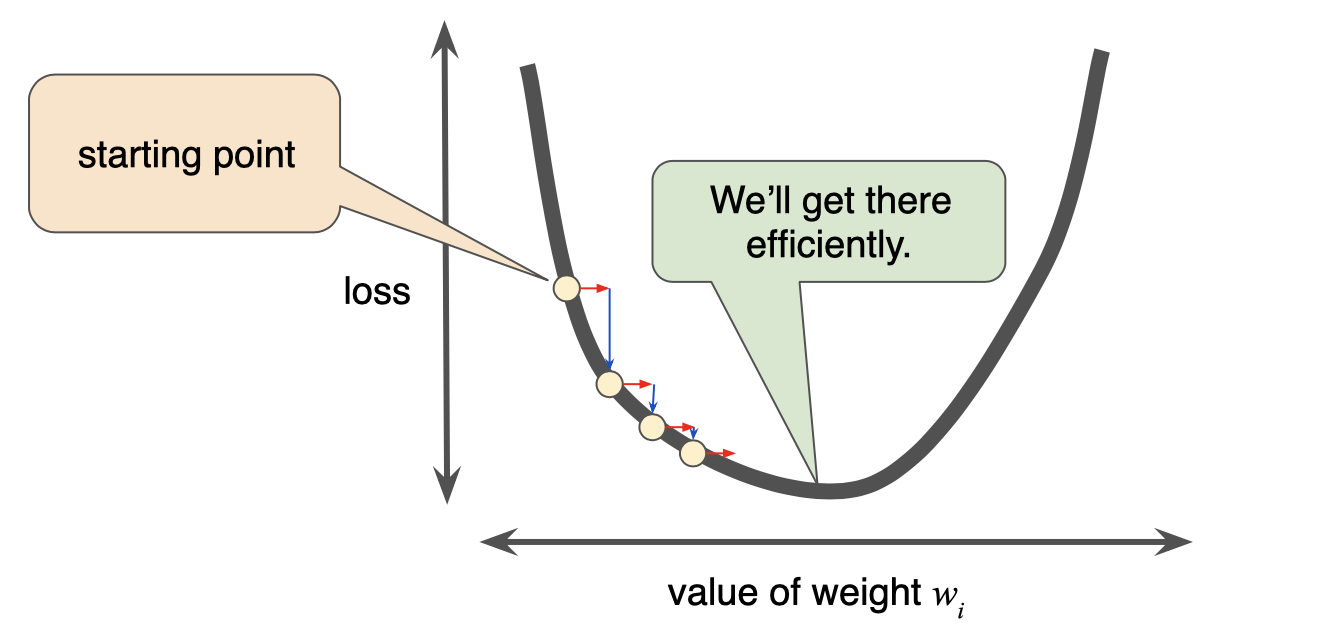
\includegraphics[scale=0.40]{final/figures/adaptive_lr.png}
        \end{figure}
\vspace*{\fill}
\textit{\tiny{(Taken from: 
\url{https://developers.google.com/machine-learning/crash-course/reducing-loss/gradient-descent})}}
\end{frame}
\begin{frame}{Stochastic Gradient Descent (SGD)}
    \begin{itemize}
        \item<1-> Use adaptive learning rate algorithms 
        \begin{itemize}
            \item<1->  AdaGrad [Duchi et al., 2011], 
            \item<1-> AdaDelta [Zeiler, 2012], 
            \item<1-> RMSProp [Tieleman and Hinton, 2012], 
            \item<1-> Adam [Kingma and Ba, 2014] 
        \end{itemize}
        \item<2-> these methods train usually faster than SGD
        \item<3-> found solution is often not as good as that by SGD $\rightarrow$ First train with Adam, fine-tune with SGD
        \item<4-> they use different initial parameter values in different runs of experiments and report the average of scores
    \end{itemize}
\end{frame}
\begin{frame}{Backpropagation}
\begin{itemize}
    \item<1-> a fancy name for a recursive algorithm that computes the derivatives of a nested functions using the chain rule, while caching intermediary derivatives 
    \item<2-> chain rule: Assume $y = f(g(x))$
    \begin{equation*}
        \frac{\partial y}{\partial x} = \frac{\partial f}{\partial g}\times \frac{\partial g}{\partial x}   = \frac{\partial f}{\partial g}\frac{\partial g}{\partial x}
    \end{equation*}
\end{itemize}
\end{frame}
\begin{frame}{Backpropagation}
\begin{itemize}
    \item<1-> consists of two steps
    \begin{itemize}
        \item<2-> forward pass $\rightarrow$ use current parameter values to compute the loss value
        \item<3-> backward pass $\rightarrow$ use the gradient of the loss to update the parameter values
    \end{itemize}
\end{itemize}
\end{frame}
\begin{frame}{Backpropagation: Forward Pass}
    \centering
    \begin{tikzpicture}
        \uncover<1->{
        \node[] (x) at (0,0) {x};
        \node[draw, minimum height=2, minimum width=3] (l1) at (0,1) {f \left( xW^{(1)} \right)$};
        \draw[->, thick] (x) -- (l1);
        \node[] (h1) at (0,2) {$h^{(1)}$}; 
        \draw[->, thick] (l1) -- (h1);
        }
    \uncover<2->{
        \node[draw, minimum height=2, minimum width=3] (l2) at (0,3) {$ f\left( h^{(1)}W^{(2)} \right)$};
        \draw[->, thick] (h1) -- (l2);
        \node[] (h2) at (0,4) {$h^{(2)}$}; 
        \draw[->, thick] (l2) -- (h2);
        }
     \uncover<3->{
        \node[draw, minimum height=2, minimum width=3] (l3) at (0,5) {$ f \left( h^{(2)}W^{(3)} \right)$};
        \draw[->, thick] (h2) -- (l3);
        \node[] (y_hat) at (0,6) {$\hat{y}$}; 
        \draw[->, thick] (l3) -- (y_hat);
        }
        \uncover<4->
        {
        \node[] (comma) at (0,6.5) {$,$};
        \node[] (y) at (0,7) {$y$}; 
        \node[draw, dashed,thick, circle] (loss) at (5,7) {$L(y,\hat{y})$};
        \draw[->, thick, dashed] (y) -- (loss);
        \draw[->, thick, dashed] (y_hat) -- (loss);
        }
        
    \end{tikzpicture}
\end{frame}
\begin{frame}{Backpropagation: Backward Pass}
    \centering
    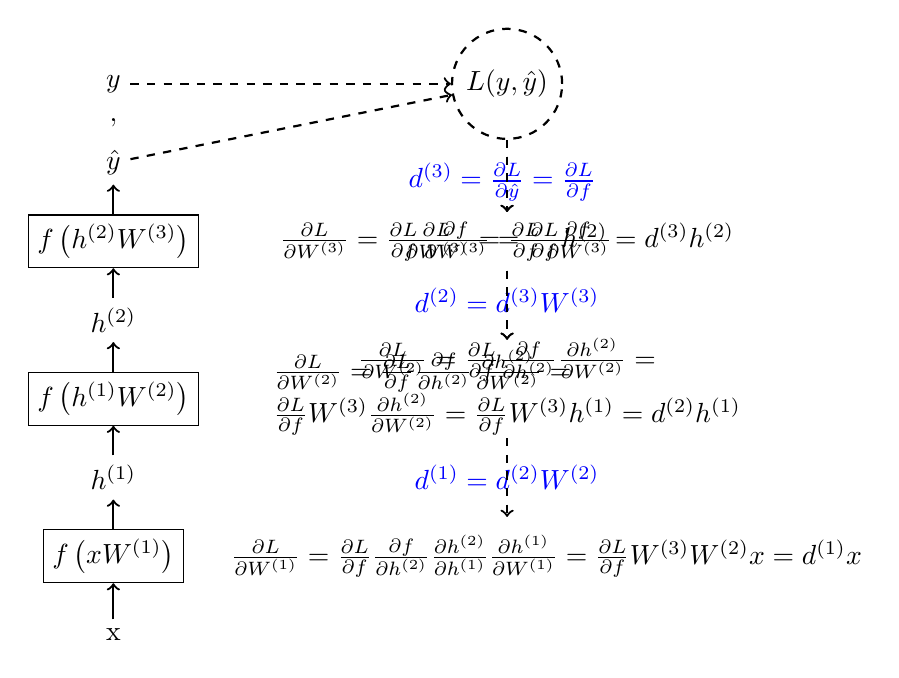
\begin{tikzpicture}
        \uncover<1->{
        \node[] (x) at (0,0) {x};
        \node[draw, minimum height=2, minimum width=3] (l1) at (0,1) {$f \left( xW^{(1)} \right)$};
        \draw[->, thick] (x) -- (l1);
        \node[] (h1) at (0,2) {$h^{(1)}$}; 
        \draw[->, thick] (l1) -- (h1);
        }
    \uncover<1->{
        \node[draw, minimum height=2, minimum width=3] (l2) at (0,3) {$ f \left( h^{(1)}W^{(2)} \right)$};
        \draw[->, thick] (h1) -- (l2);
        \node[] (h2) at (0,4) {$h^{(2)}$}; 
        \draw[->, thick] (l2) -- (h2);
        }
     \uncover<1->{
        \node[draw, minimum height=2, minimum width=3] (l3) at (0,5) {$ f \left( h^{(2)}W^{(3)} \right)$};
        \draw[->, thick] (h2) -- (l3);
        \node[] (y_hat) at (0,6) {$\hat{y}$}; 
        \draw[->, thick] (l3) -- (y_hat);
        }
        \uncover<1->
        {
        \node[] (comma) at (0,6.5) {$,$};
        \node[] (y) at (0,7) {$y$}; 
        \node[draw, dashed,thick, circle] (loss) at (5,7) {$L(y,\hat{y})$};
        \draw[->, thick, dashed] (y) -- (loss);
        \draw[->, thick, dashed] (y_hat) -- (loss);
        }
        \uncover<2->
        {
        
        \node[] (d3) at (5,5.75) {\textcolor{blue}{$d^{(3)} = \frac{\partial L}{ \partial \hat{y}} = \frac{\partial L}{ \partial f}$ }}; 
        }
        \uncover<3-3>
        {
        \node[] (d2_grad) at (5,5) 
        {$
         \frac{\partial L}{\partial W^{(3)}} = \frac{\partial L}{\partial f} \frac{\partial f}{\partial W^{(3)}}
        $}; 
        \draw[dashed, thick,->] (loss) -- (d2_grad);
        }
        
        \uncover<4->
        {
        \node[] (d3) at (5,5) 
        {$
         \frac{\partial L}{\partial W^{(3)}} = 
        \frac{\partial L}{\partial f} \frac{\partial f}{\partial W^{(3)}} =
        \frac{\partial L}{\partial f} h^{(2)} = d^{(3)}h^{(2)}
        $}; 
        \draw[dashed, thick,->] (loss) -- (d2_grad);
        }
        
        \uncover<5->
        {
        
        \node[] (d2) at (5,4.25) 
        {
      \textcolor{blue}{ $d^{(2)} = d^{(3)}W^{(3)}$}
        };
        }
        \uncover<6-6>
        {
        \node[] (d2) at (5,3.5) 
        { 
        
        $
        \frac{\partial L}{\partial W^{(2)}} = 
        \frac{\partial L}{\partial f} \frac{\partial f}{\partial h^{(2)}} \frac{\partial h^{(2)}}{\partial W^{(2)}} = 
        $             

        }; 
      \draw[->, dashed, thick] (d3) -- (5,3.75);
        }
    \uncover<7->
        {
        
        \node[] (d2) at (5,3.5) 
        { 
        \begin{tabular}{l}
        \\
        \\
        $
         \frac{\partial L}{\partial W^{(2)}} = 
        \frac{\partial L}{\partial f} \frac{\partial f}{\partial h^{(2)}} \frac{\partial h^{(2)}}{\partial W^{(2)}} = 
        $             
        \\
        $ 
        \frac{\partial L}{\partial f} W^{(3)} \frac{\partial h^{(2)}}{\partial W^{(2)}} = 
        \frac{\partial L}{\partial f} W^{(3)} h^{(1)} = d^{(2)}h^{(1)}
        $
   
        \end{tabular}
        }; 
      \draw[->, dashed, thick] (d3) -- (5,3.75);
        
        }
        
    \uncover<8->
    {
    \node[] (d2) at (5,2) 
        {
      \textcolor{blue}{ $d^{(1)} = d^{(2)}W^{(2)}$}
        };
    }
    \uncover<9->
        {
        
        \node[] (d1) at (5.5,1) 
        { 
        $
         \frac{\partial L}{\partial W^{(1)}} = 
        \frac{\partial L}{\partial f} \frac{\partial f}{\partial h^{(2)}} \frac{\partial h^{(2)}}{\partial h^{(1)}}
        \frac{\partial h^{(1)}}{\partial W^{(1)}}
        = 
        \frac{\partial L}{\partial f} W^{(3)}  W^{(2)} x = d^{(1)} x 
        $
 
        }; 
         \draw[->, dashed, thick] (5,2.5) -- (5,1.5);
        }
    \end{tikzpicture}
\end{frame}
\begin{frame}{Backprop + SGD}
\begin{itemize}
    \item<1-> the output of backprop is gradient of parameters of a neural model
    \item<2-> once we have the gradients we can use SGD rule to update the parameter values
\end{itemize}
\end{frame}
\begin{frame}[fragile]{A Simple Training Loop in PyTorch}
\begin{lstlisting}[language=Python]
optimizer = SGD(model_params, lr)

for epoch in range(num_epochs):
    for x,y in  data_batches:
        
        y_hat = model(x) 
        loss = loss_func(y_hat, y)
        
        optimizer.zero_grad() 
        loss.backward()
        
        optimizer.step()
\end{lstlisting}
\end{frame}